\documentclass[../main.tex]{subfiles}
\begin{document}
\subsubsection{Stochastic perturbations: noise-induced (N-)tipping}\label{subsubsec3.1.3}
One substantially strong assumption that we need to discard in order to build a more realistic dynamical system for the prediction of critical transition is the deterministic character of its dynamics.
Whether it is due to the intrinsic stochastic nature of the phenomenon under investigation or to the noise naturally embedded in the sensory data collected in scientific monitoring, the stochastic character of real-world timeseries data is inevitable.
We thus need to move away from the classical theory of flows in ordinary differential equations (ODEs) and into the realm of stochastic processes.
In \cite{Kuehn11} the fast-slow problem \eqref{eq3.1} in the slow timescale $\tau=\varepsilon t$ is reformulated as an Itô differential form
\begin{equation}\label{eq3.6}
   \begin{cases}
      dx = \epsilon^{-1} f(x;\mu)d\tau + \frac{\sigma_f}{\sqrt{\epsilon}}\,dW\,, \\
      d\mu = g(x;\mu)d\tau\,, 
   \end{cases}
\end{equation}
whith $f$ and $g$ modelling the deterministic drift of an ensemble's average of trajectories, $\sigma_{f}$ modelling the stochastic diffusion on such ensemble and $W$ representing Brownian motion.
We can now exploit the slow manifold $C_{\varepsilon}$ introduced in Theorem \ref{thm3.1} to derive a criterion to discern an ensemble's trajectory close to the critical transition from one that is in a stable regime.
According to Definition \ref{def3.1} in fact, a sample path of an ensemble of trajectories of \eqref{eq3.6} that stays close (in probabilistic terms) to $C_{\varepsilon}$ will be in a regime of slow, stable evolution.
It is thus intuitive to define a new stochastic process $\xi(\tau)=x(\tau)-h_{\epsilon}(\mu)$ which quantifies the statistical departure of the sample path $x(\tau)$ from the critical manifold. 
We then apply Ito's formula to this new process to derive the associated SDE; after that we define once again a new stochastic process $X(\tau):=\sigma_f^{-2} \text{Var}(\xi)$ which satisfies the following deterministic fast-slow system
\begin{equation}\label{eq3.7}
   \begin{cases}
      \dot{X} = 2\epsilon^{-1}A_{\epsilon}(\mu)X +1 \,, \\
      \dot{\mu} = g(h_{\epsilon}(\mu),\mu) \,, 
   \end{cases}
\end{equation}
with $A_{\epsilon}(\mu)=(D_x f)(h_{\epsilon}(\mu),\mu) - \epsilon (D_{\mu} h_{\epsilon})(\mu) (D_x g)(h_{\epsilon}(\mu),\mu)$. 
Applying Theorem \ref{thm3.1} again for \eqref{eq3.7} we can construct a new slow manifold for the sample paths of the new stochastic fast-slow system
\begin{equation}\label{eq3.8}
        C_{\epsilon}^{(X)}:=\bigg\{(X,\mu)\in \mathbb{R}^2\;:\;X=H_{\epsilon}(\mu):=- \frac{1}{2A_{\epsilon}(\mu)+O(\epsilon)}\bigg\}\,,
\end{equation}
and from that we finally can define a neighbour of the slow manifold which scales with the variance of sample paths
\begin{equation}\label{eq3.9}
        N_{\rho}(C_{\epsilon}):=\bigg\{(x,\mu)\in \mathbb{R}^{2}\;:\;\frac{(x-h_{\epsilon}(\mu))^{2}}{H_{\epsilon}(\mu)}<\rho^2\bigg\}\,.
\end{equation}
We formalise the above derivation in the Theorem below.
\begin{theorem}[label=thm3.4]{}{}
        Let \eqref{eq3.6} be a scalar stochastic fast-slow system (i.e. $n=m=1$) with additive noise (i.e. $\sigma_{f}(x)=\sigma\in \mathbb{R}$) and 
     \begin{equation*}
             N_{\rho}(C_{\varepsilon}):=\bigg\{(x,\mu)\in \mathbb{R}^{2}\;:\;-\frac{(x-h_{\varepsilon}(\mu))^{2}}{2A_{\varepsilon}(\mu)+\mathcal{O}(\varepsilon)}<\rho^2\bigg\}\,,\quad A_{\varepsilon}(\mu)=(D_x f)(h_{\varepsilon},\mu) - \varepsilon (D_{\mu} h_{\varepsilon}) (D_x g)(h_{\varepsilon},\mu)\,,
     \end{equation*}
     be a neighbour of the singularly perturbed slow manifold, then if a sample path has an initial condition on the slow manifold $C_{\varepsilon}$ it will stay bounded within $N_{\rho}(C_{\varepsilon})$ with high probability.
\end{theorem}
Arguably of greater importance for the context of EWS detection is the corollary that follows.
\begin{corollary}
     Since the measure of $N_{\rho}(C_{\varepsilon})$ scales with the variance of $\xi(\tau)$ (which coincides with the variance of $x(\tau)$ from trivial properties of the variance of a sum of stochastic processes) then an increase in the variance implies the neighbour to grow bigger.
\end{corollary}
Whenever a stochastic process tracking a (deterministic) slow stable manifold is \textit{kicked-off} due to the perturbations of the noise and escapes the basin of attraction we are presented with a case of the previously discussed N-tipping.
Despite the notorious difficulty of anticipating N-tipping events, the corollary above provides us with a robust mathematical characterisation of either CSD or flickering through the increase in variance of a stochastic process approaching B-tipping.
The intuition behind CSD for B-tipping is that as the bifurcation is approached the neighbor $N_{\rho}(C_{\varepsilon})$, in which the realisations of the stochastic process are bounded, increases in size allowing for more probability to a N-tipping event to occur.
\begin{example}[label=ex3.3]{}{}
In \cite{Kuehn11} an example is provided to validate this result using an OUP
\begin{equation}\label{eq3.10}
   \begin{cases}
           dx = -\varepsilon^{-1}\alpha x d\tau + \frac{\sigma}{\sqrt{\varepsilon}}dW \,, \\
      d\mu = d\tau \,, 
   \end{cases}
\end{equation}
as benchmark.
Let us consider a sample path realised by the OUP in \eqref{eq3.10} with drift constant $\alpha=1$, timescale constant $\epsilon=2\cdot10^{-2}$ and noise level $\sigma=0.1$.
We want to construct the neighborhood $N_{\rho}(C_{\varepsilon})$ and confirm that the numerical sample paths stay in fact bounded within such neighborhood with high probability. 
To do so we must first construct the (deterministic) slow manifold $C_{\varepsilon}$ and for that we need in turn to derive the map $h_{\varepsilon}(\mu)=h(\mu)+\mathcal{O}(\varepsilon)$.
With the critical manifold coinciding with the $x=0$ axis 
\begin{equation*}
            C=\{(x,\mu)\in \mathbb{R}^{2}\;:\;f(x,\mu)=-\alpha x = 0\:\Rightarrow\: x=0\;\forall \alpha\neq0,\,\forall \mu\in \mathbb{R}\}\,,
\end{equation*}
we can easily check that the existance of $h:\mu\mapsto x$ is guranteed by Theorem \ref{thm2.1} given that $C$ is normally hyperbolic at any point.
It follows similarly that the only map $x=h(\mu)=0,\:\forall \mu\in \mathbb{R}$ is the null function yielding 
\begin{equation*}
                h_{\varepsilon}(\mu) = h(\mu) + \mathcal{O}(\varepsilon) = \mathcal{O}(\varepsilon)\quad\Longrightarrow\quad C_{\varepsilon}=\{(x,\mu)\in \mathbb{R}^{2}\;:\;x=O(\varepsilon)\}\,.
\end{equation*}
This tells us that the slow manifold is a narrow strip wrapped around the critical manifold whose width is twice the Hausdorff distance from $C$.
The next step in our construction is to derive a new slow manifold $C_{\varepsilon}^{(X)}$ for the process 
\begin{equation*}
             X=\sigma^{-2}\text{Var}(\xi)=\sigma^{-2}\text{Var}(x - h_{\varepsilon}(\mu))=\sigma^{-2}\text{Var}(x)\,,
\end{equation*}
where we recall the invariance of the variance under additive constant perturbations.
First we compute the quantity $A_{\epsilon}(\mu)=(D_x f)(h_{\varepsilon}(\mu),\mu) - \varepsilon (D_{\mu} h_{\varepsilon})(\mu) (D_x g)(h_{\varepsilon}(\mu),\mu)=-\alpha$ and then by using the definition
\begin{equation*}
     C_{\varepsilon}^{(X)}:=\bigg\{(X,\mu)\in \mathbb{R}^2\;:\;X=H_{\varepsilon}(\mu):=- \frac{1}{2A_{\varepsilon}(\mu)+\mathcal{O}(\varepsilon)}\bigg\}\,,
\end{equation*}
we get
\begin{equation*}
     C_{\varepsilon}^{(X)}=\{(X,\mu)\in \mathbb{R}^{2}\;:\;X=\frac{1}{2 \alpha}+O_{1}(\varepsilon)\}\,.
\end{equation*}
Furthermore from the definition
\begin{equation*}
     N(\rho;C_{\varepsilon}):=\bigg\{(x,\mu)\in \mathbb{R}^{2}\;:\;\frac{(x-h_{\varepsilon}(\mu))^{2}}{H_{\varepsilon}(\mu)}<\rho^2\bigg\}\,,
\end{equation*}
\end{example}
\begin{example_continued}
we get
\begin{equation}\label{eq3.11}
                N(\rho;C_{\varepsilon})=\bigg\{\frac{\sigma^{-2}\text{Var}(x)+O_{2}(\varepsilon)}{\frac{1}{2 \alpha}+O_{1}(\varepsilon)}<\rho^{2}\bigg\}=\bigg\{\frac{\sigma^{-2}\text{Var}(x)+M_{2}\varepsilon}{\frac{1}{2 \alpha}+M_{1}\varepsilon}<\rho^{2}\bigg\}\,,
\end{equation}
for which $M_{1}, M_{2}$ are two distinct, positive constants that need to be quantified in order to compute $\rho$ which will give us the boundaries $\partial N(\rho;C_{\varepsilon})=\sqrt{\rho^{2}}$.
To do so let us observe that $X=H_{\varepsilon}(\mu)=\frac{1}{2A_{\varepsilon}(\mu)}+O_{1}(\varepsilon)\;\Rightarrow\;|X|=|\sigma^{-2}\text{Var}(x)|< M_{1}\varepsilon$.
We recall that $x(\tau)$ is in fact an OUP for which we have an analytical expression for its variance readily available
\begin{equation}\label{eq3.12}
             \text{Var}(x(\tau)) = \bigg(x_0 - \frac{\sigma^2}{2 \alpha}\bigg)e^{-2\frac{\alpha\tau}{\varepsilon}}\,.
\end{equation}
We can the plug in the values for $\alpha,\,\sigma$ and $\varepsilon$ in \eqref{eq3.12} to get $M_{1}=225$.
Similarly for the other constant we get $x=h_{\varepsilon}(\mu)=O_{2}\;\Rightarrow\;|x|<M_{2}\varepsilon$; here we assume that $\underset{\tau\in \mathbb{R}^{+}}{\text{max}}|x(\tau)|=0.25$ which lead us to the value $M_{2}=12.5$. Putting all together into \eqref{eq3.11} finally gives us $\rho = \pm 0.35$.
We are now able to compute the closure of the neighborhood $N(\rho;C_{\varepsilon})$ of the critical manifold $C_{\varepsilon}$ within which our sample paths $x(\tau)$ for the OUP (which are normally distributed) will stay bounded with high probability.
\begin{figure}[H]
         \centering 
         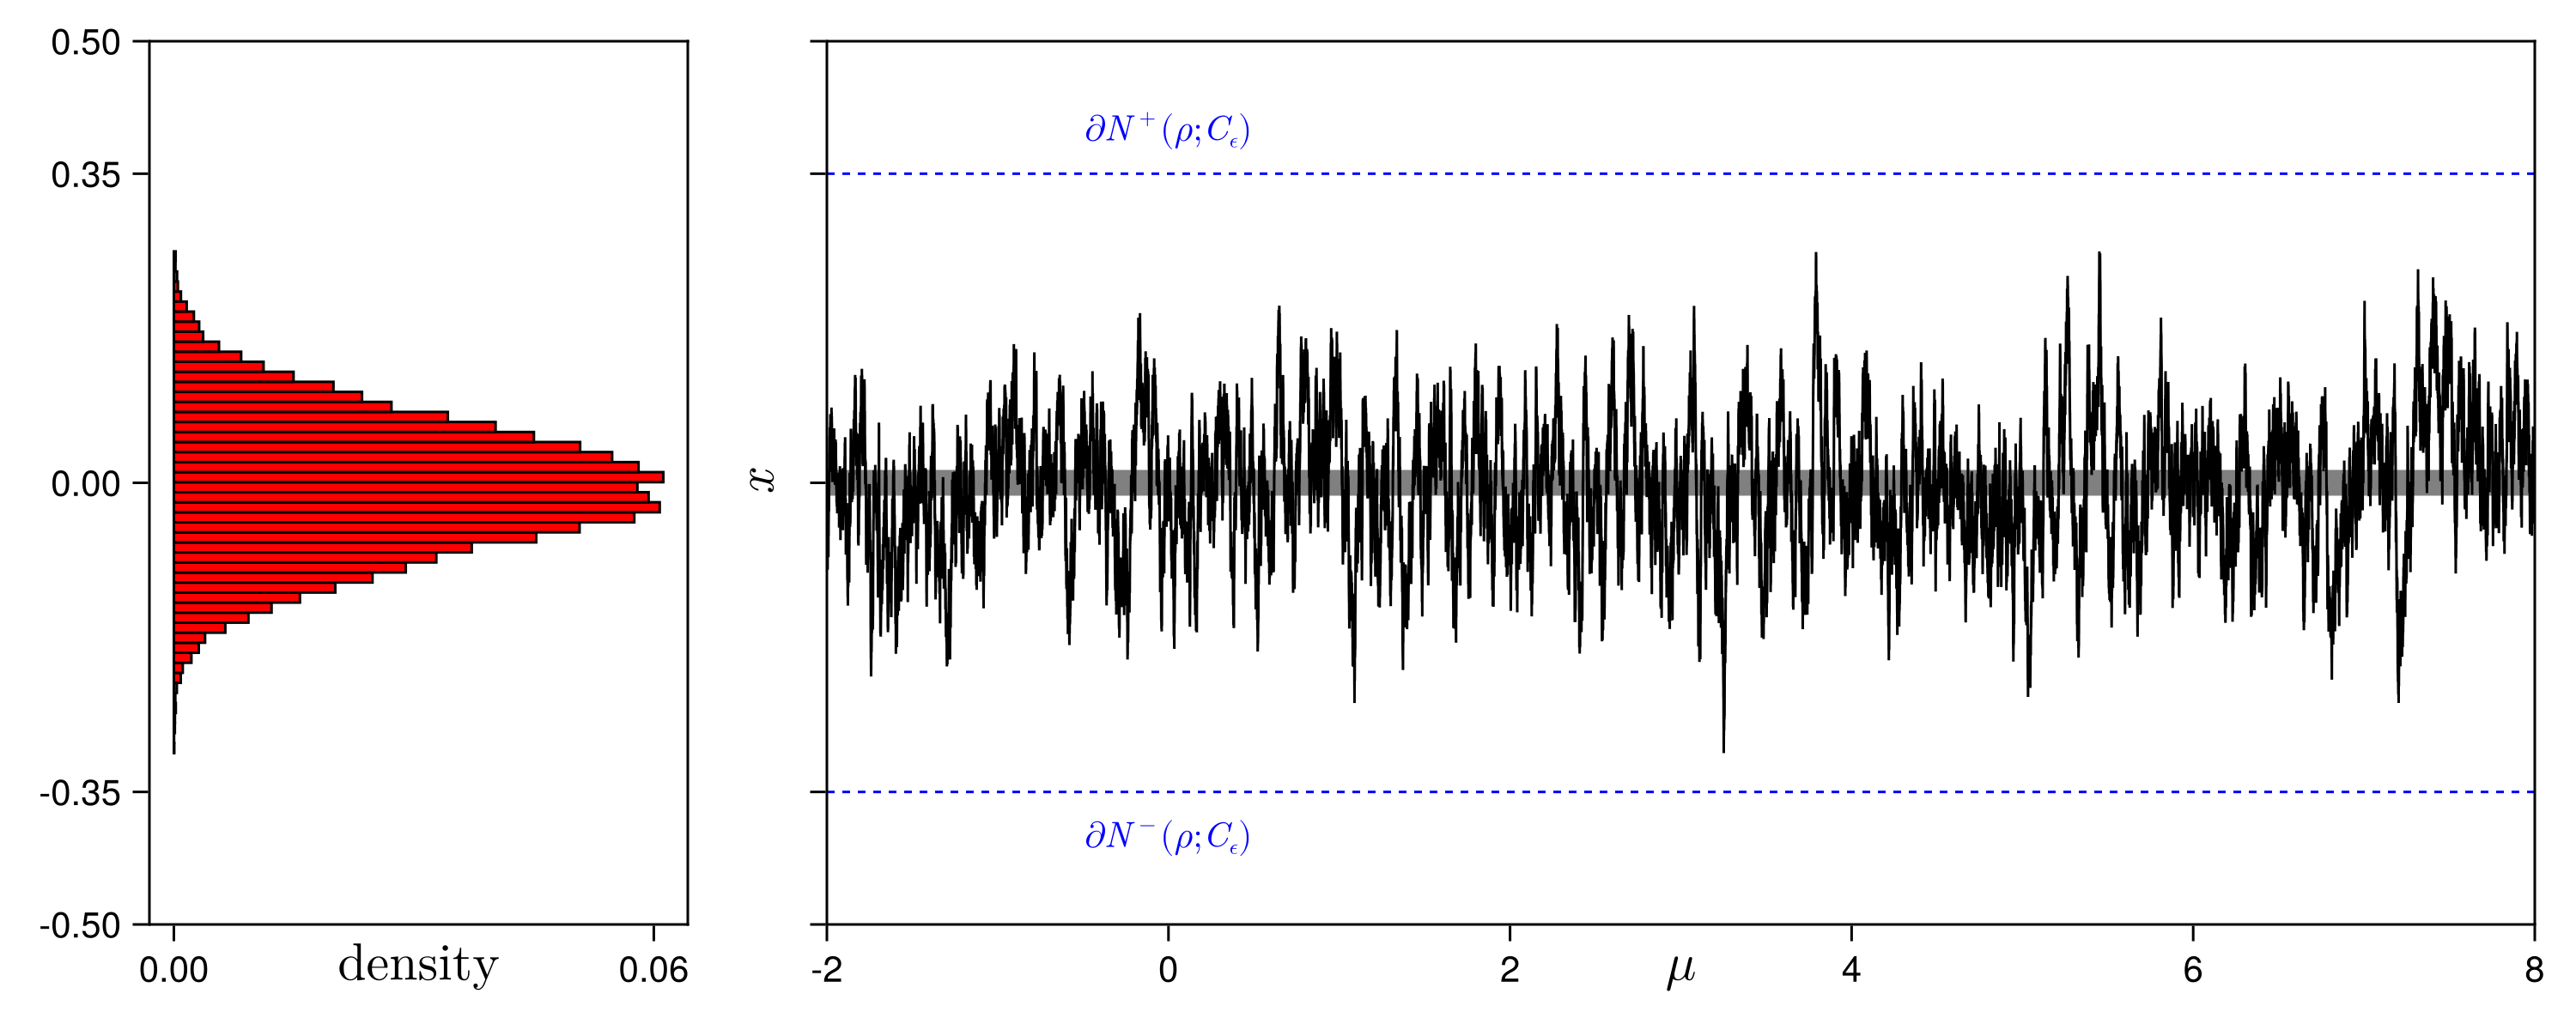
\includegraphics[keepaspectratio, width=\textwidth]{../figures/fig3.3.png}
         \caption{States distribution (left) of a sample path (right) of the OUP \eqref{eq3.10}, with drift $\alpha=1$, timescale separation $\varepsilon=2\cdot10^{-2}$ and noise level $\sigma=0.1$, starting on the slow manifold $C_{\varepsilon}$ (gray strip). 
         Note how the states stay bounded within the neighborhood $N_{\rho}(C_{\varepsilon})$ (dashed blue lines) with probability $1$.}
         \label{fig3.3}
\end{figure}
\end{example_continued}
To substantiate the result given by the corollary we can generalise the approach in detecting CSD through the increase in variance of a sample path of the fast-slow problem by computing the moments of the probability distribution solving the Fokker-Planck equation (FPE) associated to the SDE.
Considering \eqref{eq3.9} again for the case of additive noise, the FPE reads
\begin{equation}\label{eq3.13}
     \partial_{t}p(x,t) = -\partial_{x}J(x,t)\,,\quad J(x,t):= f(x;\mu)p(x,t) - \frac{\sigma^{2}}{2}\partial_{x}p(x,t) \,,
\end{equation}
where $J(x,t)$ is the probability density current.
The fundamental assumption of the analysis carried in \cite{Kuehn11} is that there exist an asymptotic steady-state $x_{s}$ whose distribution $p_{s}(x):=p(x_{s},t)$ satisfies the stationary limit of \eqref{eq3.13} i.e. $\newprime{J}(x) = 0\;\Rightarrow\; J(x) = \text{constant}(x)$. 
We immediately realise that equation \eqref{eq3.13} is defined over the entirety of the real (spatial) domain, meaning that in order to restrict it to a bounded and limited subinterval $[a,b]\subset \mathbb{R}$ we must enforce the entirety of the probability current to never leave such domain, resulting in the specification of reflecting boundary conditions. 
The reason for this immediately follow by the constraint of the stationary Fokker-Planck density to remain normalised in any subdomain $[a,b]$ we restrict ourselves to.
Following the imposition of reflecting boundary conditions we get that the only possible constant that satisfies \eqref{eq3.13} is $J(x)=J=0$. From the definition of $J(x,t)$ this leads to a first-order, homogeneous, non-linear ODE whose general integral can be explicitly calculated
\begin{equation}\label{eq3.14}
     p_{s}(x)=\frac{1}{N}\,e^{2 \int_{a}^{x}\sigma^{-2}f(y;\mu)dy}\,,\quad N = \int_{a}^{b}\int_{a}^{z}\sigma^{-2}f(y;\mu)dy\,dz\,.
\end{equation}
We can now analytically derive the variance from \eqref{eq3.14} for simple forms of the drift $f(x;\mu)$. In \cite{Kuehn11} this is done for the saddle-node, transcritical and subcritical pitchfork normal forms and we compare those with the ensemble variance of $1000$ sample paths as reported in Figure \ref{fig3.5}.
One clear observation that we can gather from Figure \ref{fig3.5} is that in all three cases the (analytic) variance is non-monotonic and it reaches a local maxima in the proximity of the bifurcation at $\mu=0$ before decreasing. 
This apparent anomaly is a result of imposing reflecting boundary conditions for the probability current.
As we previously established in fact, the approach of a critical transition implies that the stationary density $p_{s}(x)$ becomes less confined around the stable equilibrium leading to N-tipping to occur with higher and higher probability.
\begin{figure}[H]
    \centering 
    \begin{subfigure}[b]{0.3\textwidth}
        \centering 
        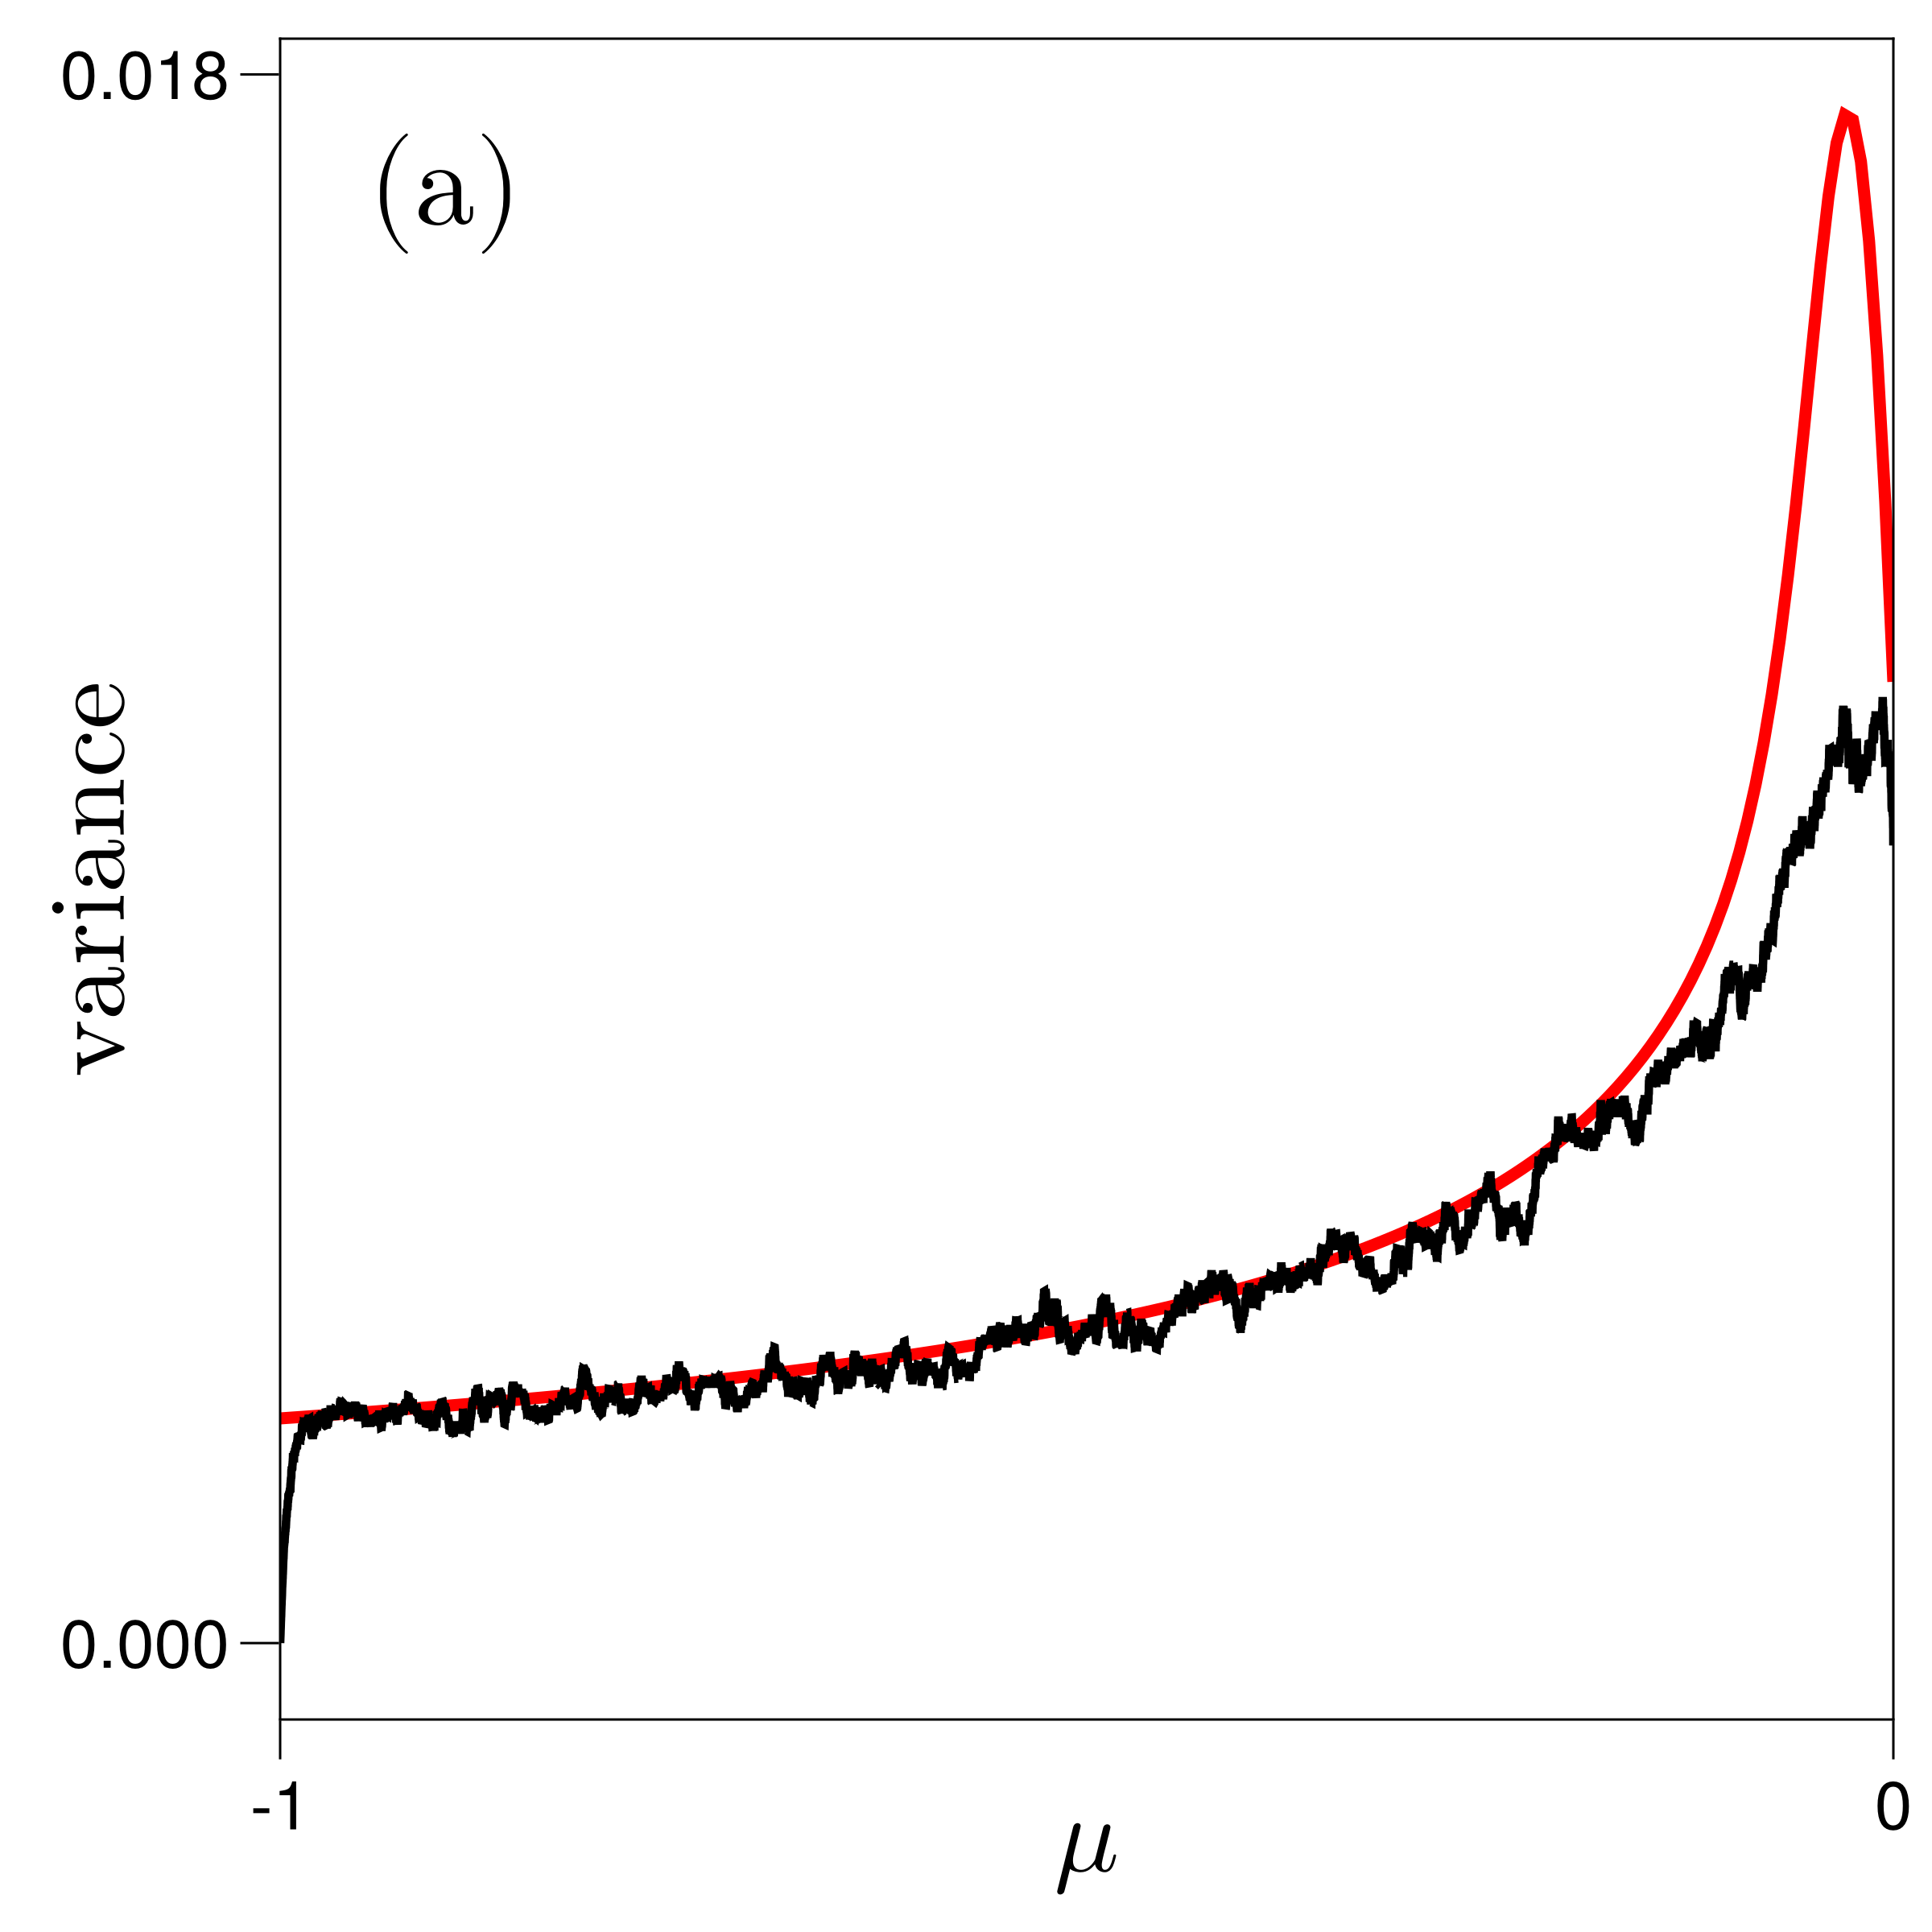
\includegraphics[keepaspectratio, width = \textwidth]{../figures/fig3.5.1.png}
        \label{fig3.5.1}
    \end{subfigure}
    \hfill 
    \begin{subfigure}[b]{0.3\textwidth}
        \centering 
        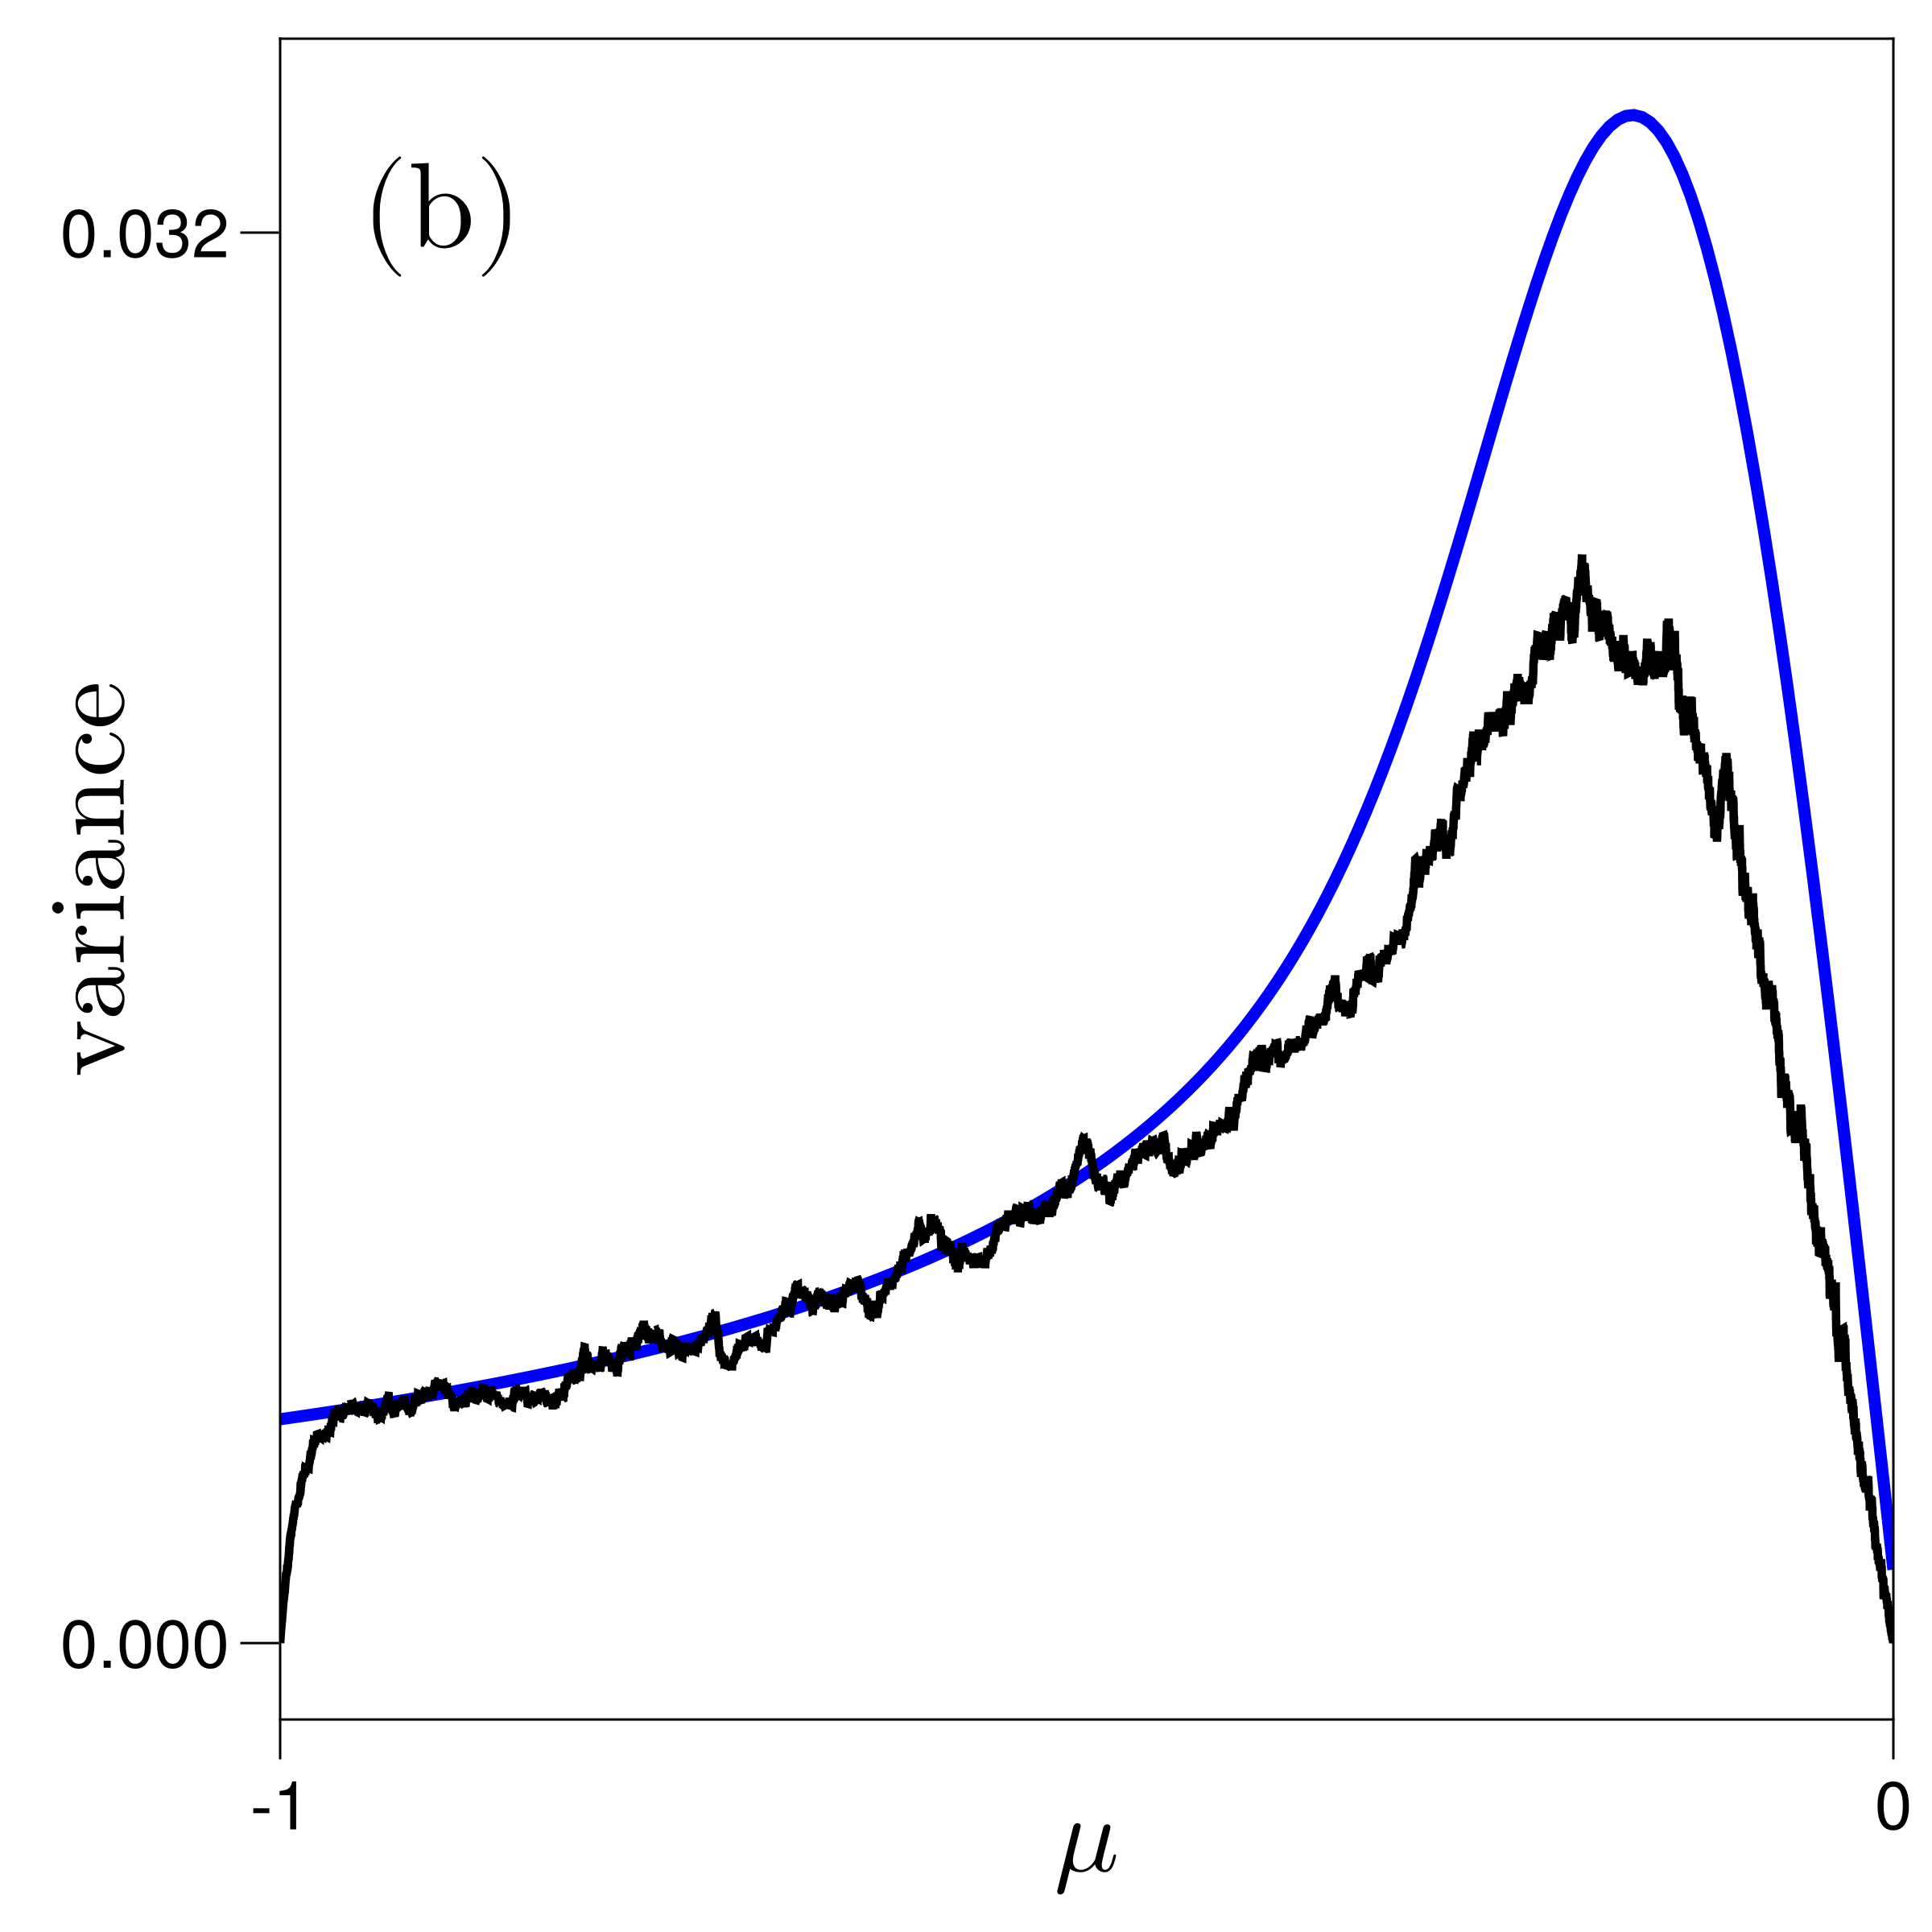
\includegraphics[keepaspectratio, width = \textwidth]{../figures/fig3.5.2.png}
        \label{fig3.5.2}
    \end{subfigure}
    \hfill
    \begin{subfigure}[b]{0.3\textwidth}
        \centering 
        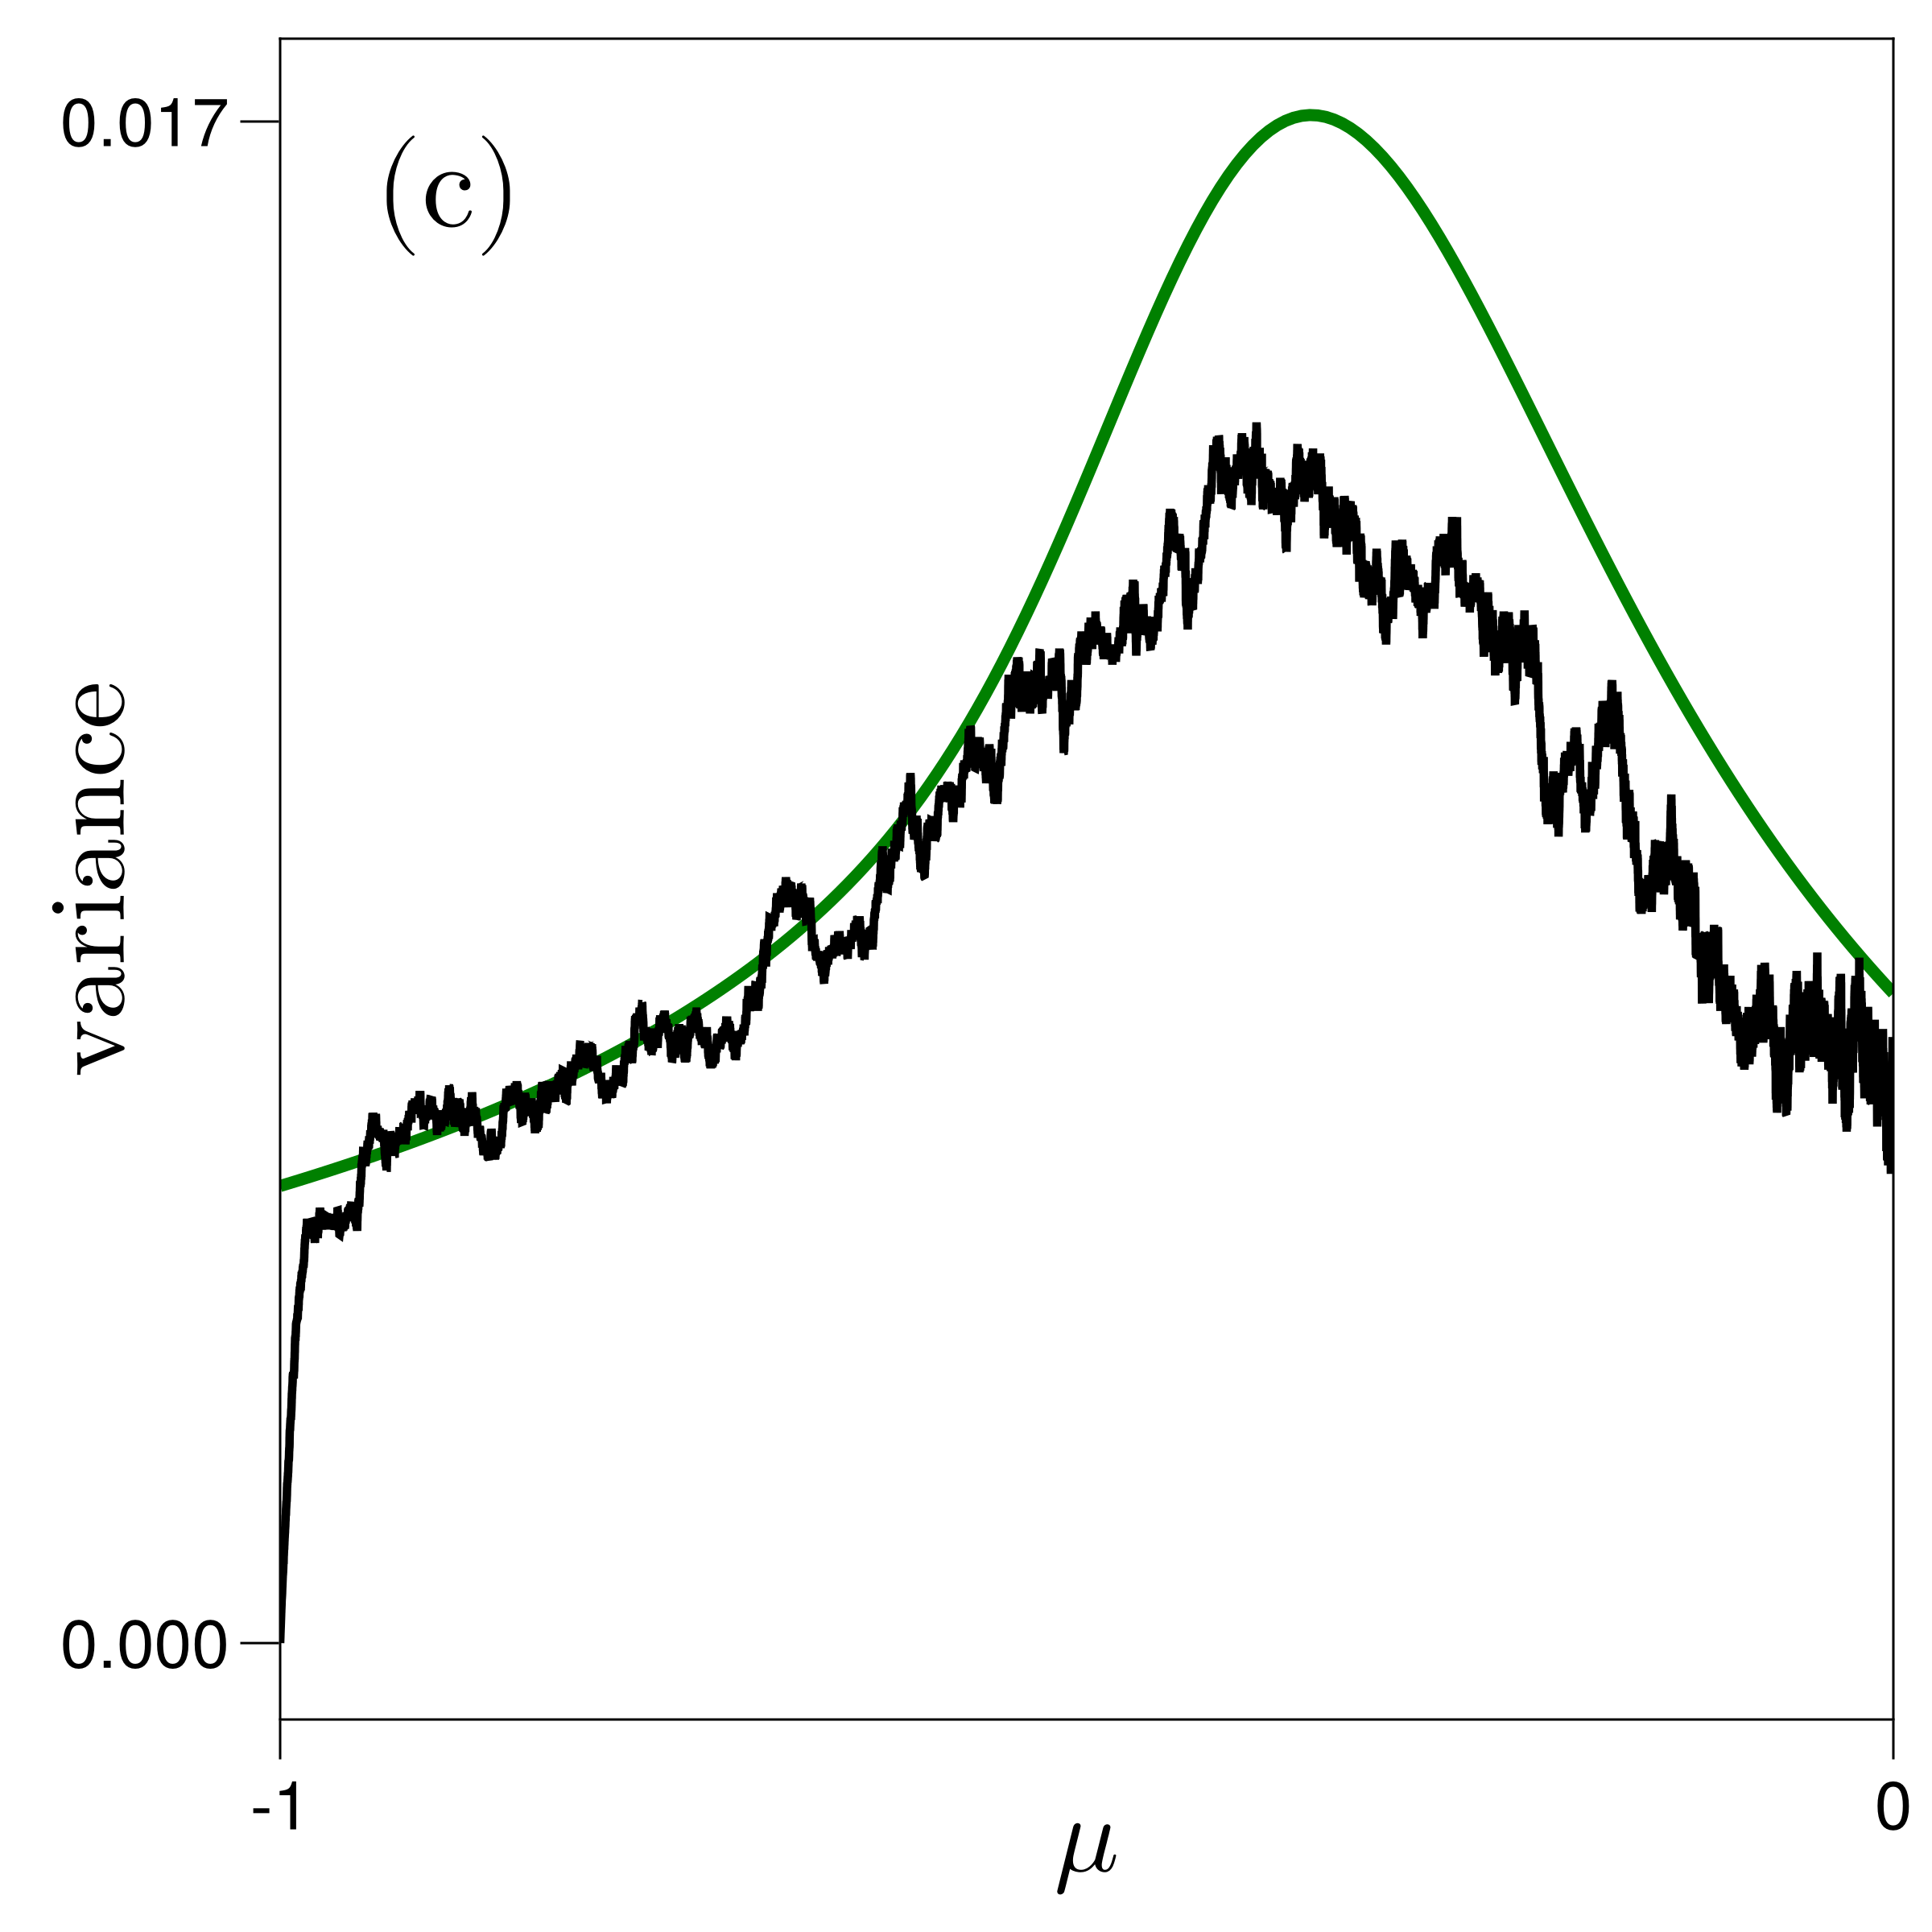
\includegraphics[keepaspectratio, width = \textwidth]{../figures/fig3.5.3.png}
        \label{fig3.5.3}
    \end{subfigure}
    \caption{Comparison between the analytical variance of the stationary Fokker-Planck distribution of the saddle-node (a), pitchfork (b) and transcritical (c) normal forms (colored lines) against the numerical variance of an ensemble of $1000$ sample paths (black lines) for the same cases (noise level $\sigma = 0.1$).}
    \label{fig3.5}
\end{figure}
The second most evident observation concerns the discrepancies between the analytical and numerical variance near the local maxima. In all three cases in fact we observe that the two curves agree when the parameter's values are far away from the deterministic critical transition however they largely differ as the parameter value gets closer to the local maxima for the analytical variance.
We can ascribe such discrepancy to (a) the choice that we made in counting the ensemble's sample paths as escaped (i.e. in counting N-tipping events) the exact moment they cross the unstable branch of the critical manifold and (b) the fact that while the analytical variance of the FPE is derived in the singular limit $\varepsilon=0$ (due to the stationarity assumption) the ensemble variance is computed within the fast-slow framework.
The first condition (a) actually imposes absorbing boundary conditions to our FPE which quite substantially differ from the reflecting boundary conditions used in the analytical derivation especially when boundary and noise effects become dominant (i.e. close to the deterministic critical transition as the basin of attraction shrinks further and further in size).
The second condition (b) emphasizes as the solution of the reduced equation in the singular limit is only an approximation of the full fast-slow dynamics.
This argument is validated further by observing how the discrepancy between the analytical and numerical variance for the saddle-node bifurcation is significantly less than those for the remaining two normal forms; based on this observation we expect fewer trajectories to escape the stable equilibrium for the saddle-node normal form and this is exactly what we observe in the ensemble simulations as depicted below in Figure \ref{fig3.6}.
\begin{figure}[H]
    \centering 
    \begin{subfigure}[b]{0.95\textwidth}
        \centering 
        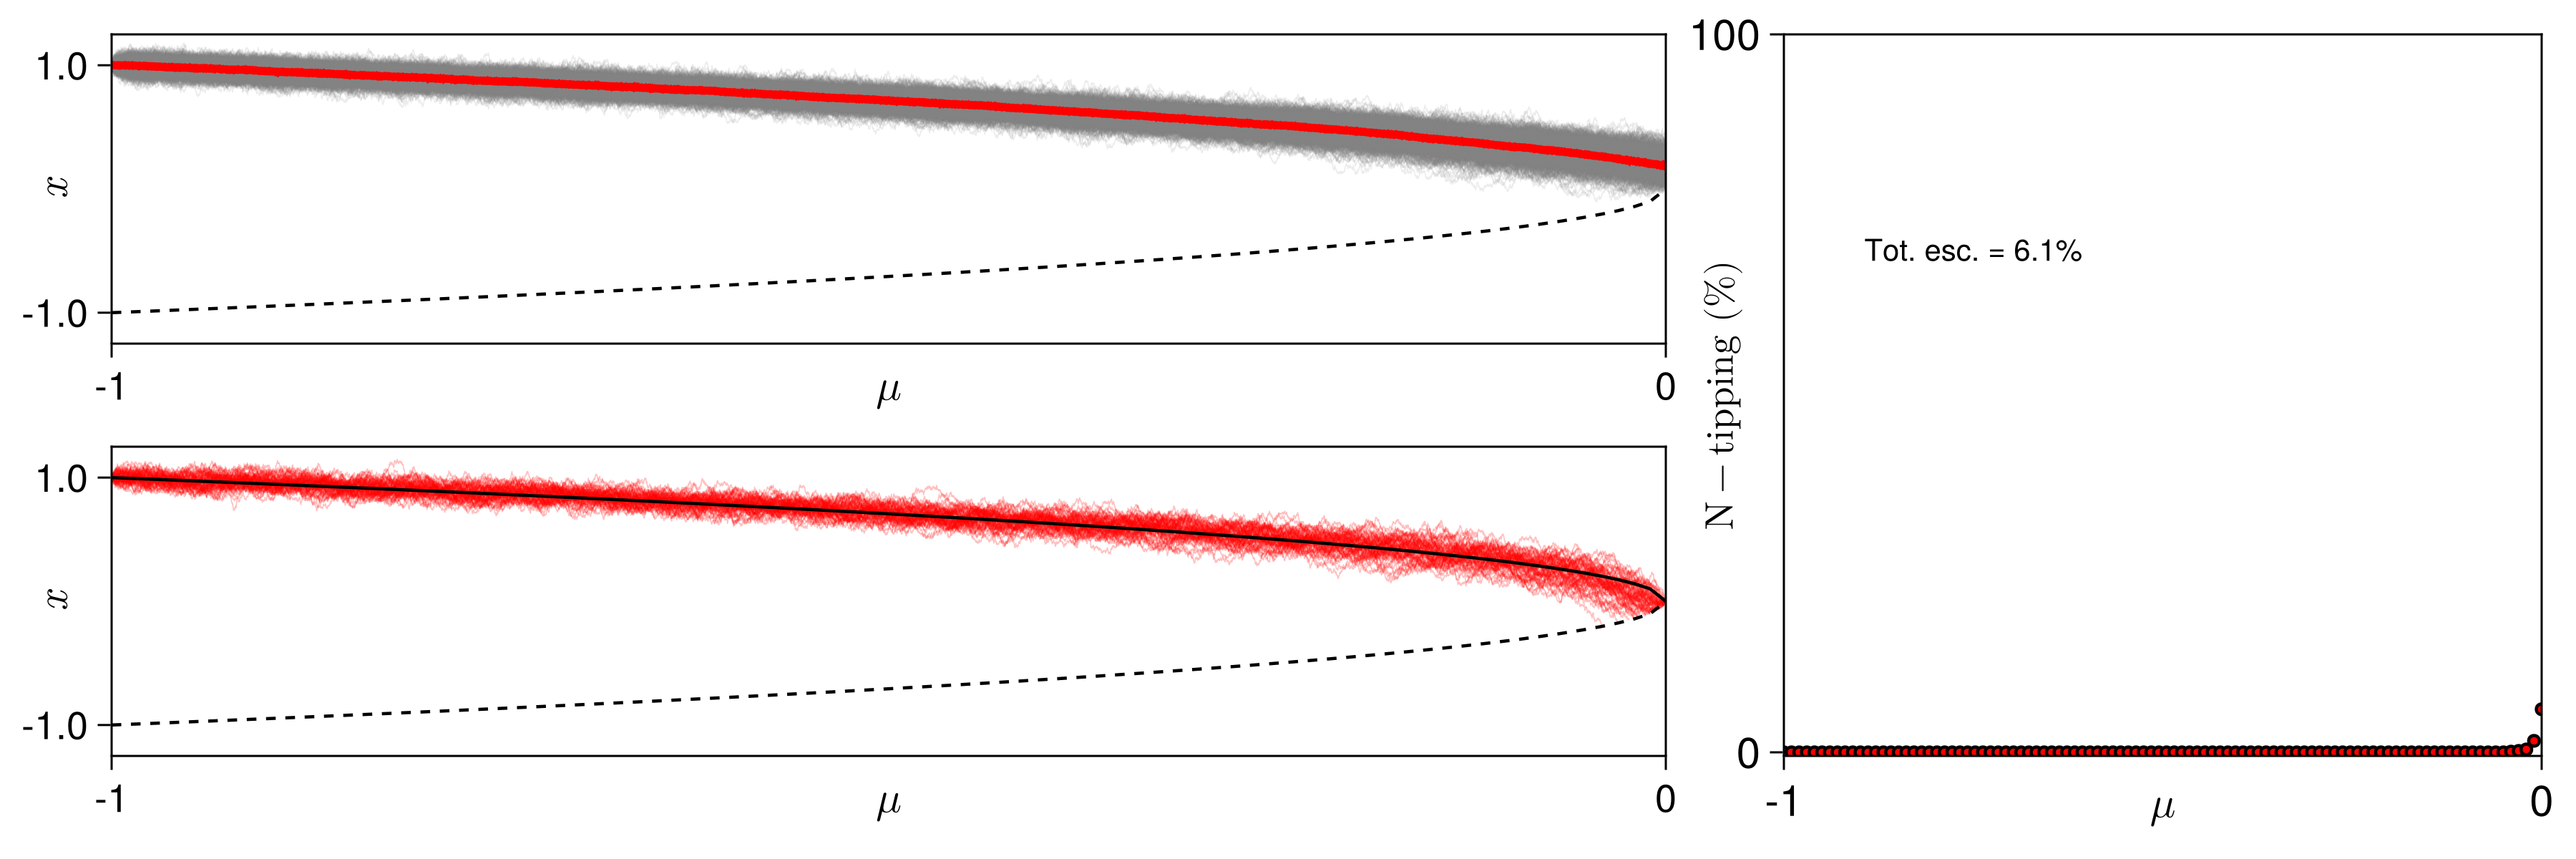
\includegraphics[keepaspectratio, width = \linewidth]{../figures/fig3.6.1.png}
        \label{fig3.6.1}
    \end{subfigure}
    \hfill 
    \begin{subfigure}[b]{0.95\textwidth}
        \centering 
        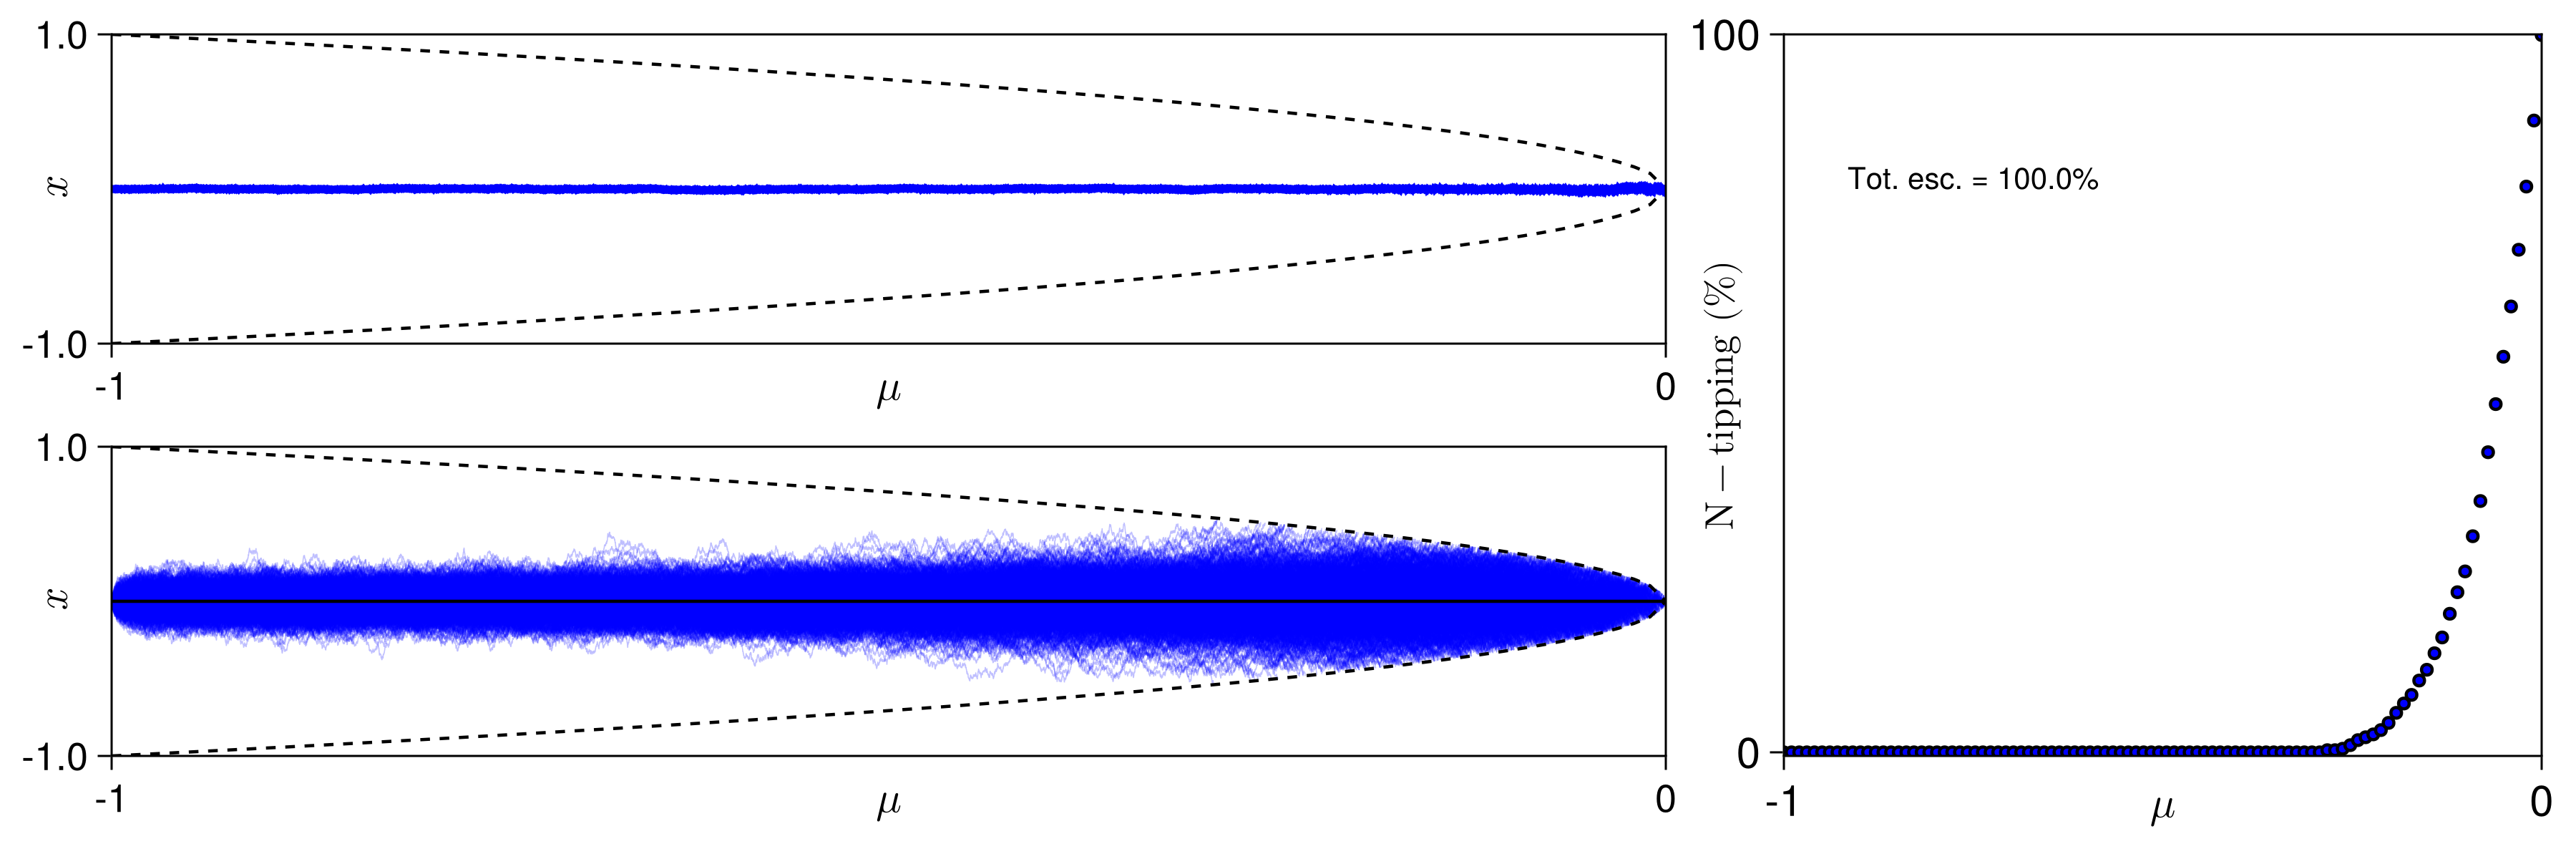
\includegraphics[keepaspectratio, width = \linewidth]{../figures/fig3.6.2.png}
        \label{fig3.6.2}
    \end{subfigure}
    \hfill
    \begin{subfigure}[b]{0.95\textwidth}
        \centering 
        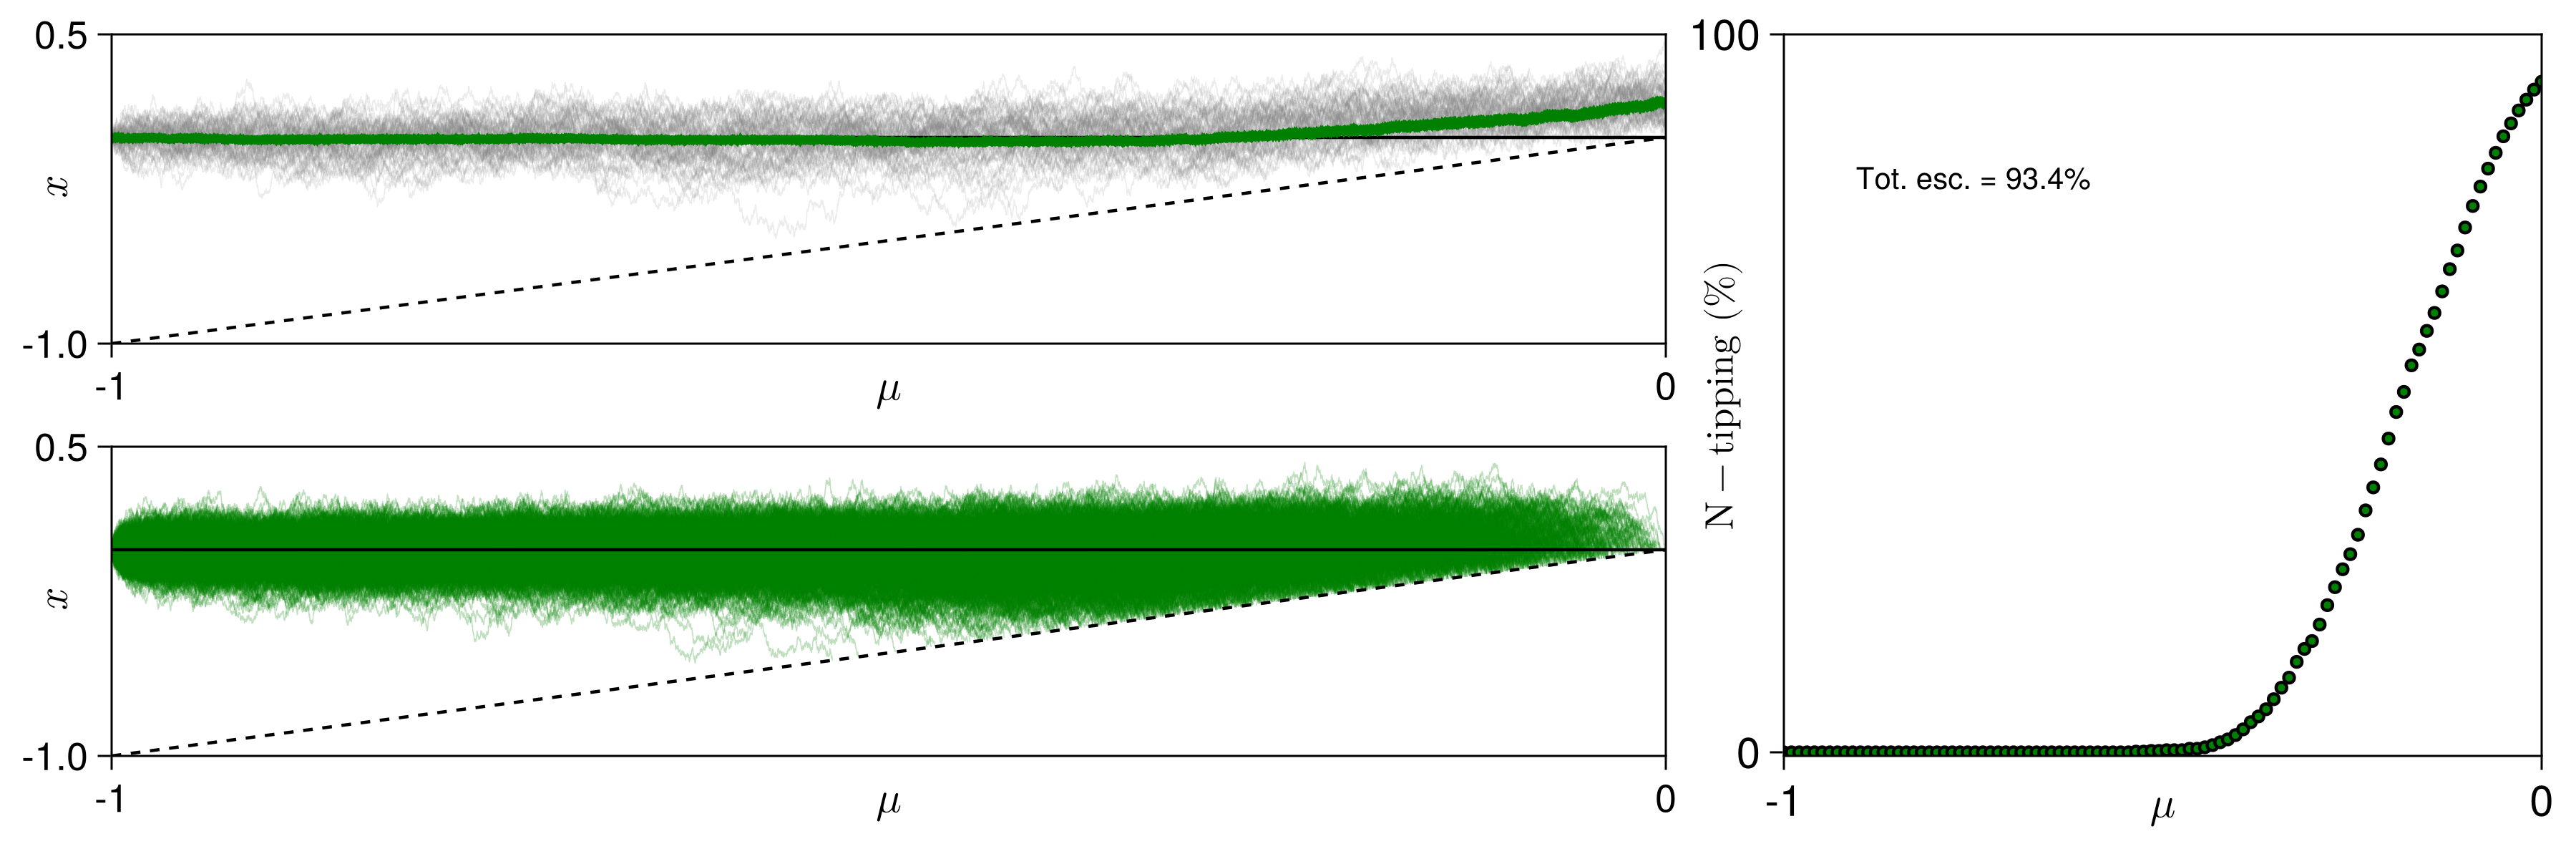
\includegraphics[keepaspectratio, width = \linewidth]{../figures/fig3.6.3.png}
        \label{fig3.6.3}
    \end{subfigure}
    \caption{Ensemble sample paths of saddle-node (top), pitchfork (middle) and transcritical (bottom) normal forms showing the trajectories that stayed bounded on the stable branch of the critical manifold (top panels: gray lines indicate the ensembles trajectories and the colored lines show the ensemble mean) and those that escaped due to N-tipping (bottom panels). 
    On the left of each plot a percentage of the number of escaped trajectories as $\mu$ vaires is shown.}
    \label{fig3.6}
\end{figure}
\begin{example}[label=ex3.4]{}{}
Consider the case of a transcritical normal form with multiplicative noise
\begin{equation*}
         dx = (\mu x - x^{2} + \frac{1}{2}\sigma^{2}x)\,dt + \sigma x\,dW\,,
\end{equation*}
as presented in \cite{Kuehn11}. 
We write the associated FPE which, in the singular limit, it reads
\begin{equation*}
          0 = -\frac{d}{dx}((yx - x^{2} + \frac{1}{2}\sigma x)p_{s}(x; y)) + \frac{d^{2}}{dx^{2}}(\frac{1}{2}\sigma^{2}x^{2}\,p_{s}(x; y))\,.
\end{equation*}
One normalizable solution of the above stationary FPE is
\begin{equation*}
          p_{s}(x) = \frac{1}{N_{\mu}}\,x^{\frac{2\mu}{\sigma^{2}}-1}\,e^{-\frac{2x}{\sigma^{2}}}\,,\quad N_{\mu}=\int_{0}^{+\infty} x^{\frac{2\mu}{\sigma^{2}}-1}\,e^{-\frac{2x}{\sigma^{2}}}\,dx = \bigg(\frac{\sigma^{2}}{2}\bigg)^{\frac{2\mu}{\sigma^{2}}}\,\Gamma\bigg(\frac{2\mu}{\sigma^{2}}\bigg)\,.
\end{equation*}
We recall the definition of the $\Gamma-$probability density function
\begin{equation}\label{eq3.15}
     f_{\alpha,\beta}(x):=\frac{1}{\Gamma(\alpha)}x^{\alpha-1}e^{-\beta x}\beta^{\alpha}
\end{equation}
where $\Gamma(z):=\int_{0}^{\infty}y^{z-1}e^{-y}dy$ is the Euler's Gamma function for $z\in \mathbb{C}$ while $\alpha,\beta\in \mathbb{R}$ parametrise the distribution.
The first central moments of \eqref{eq3.14} are well known, in particular
\begin{equation}\label{eq3.16}
     \mathbb{E}_{f}(x;\alpha,\beta) = \frac{\alpha}{\beta}\,,\quad \text{Var}_{f}(x;\alpha,\beta)=\frac{\alpha}{\beta^{2}}\,.
\end{equation}
With a simple change of variables we immediately verify that the normalised solution of the FPE of the transcritical stochastic process with linear, multiplicative noise, is equivalent to \eqref{eq3.14}
\begin{equation*}
    \alpha = \frac{2\mu}{\sigma^{2}}\,,\quad \beta=-\frac{2}{\sigma^{2}}\,. 
\end{equation*}
Putting the above into \eqref{eq3.16} yields
\begin{equation*}
     \mathbb{E}_{p_{s}}(x;\mu)=\mu\,,\quad \text{Var}_{p_{s}}(x;\mu)=\frac{\sigma^{2}}{2}\mu\,.
\end{equation*}
What is left to verify is that under the above change of variables the normalisation constant $N_{\mu}$ coincides with that of the $\Gamma-$distribution.
We write
\begin{equation*}
     N_{\mu}=\int_{0}^{\infty}x^{\frac{2\mu}{\sigma^{2}}-1}e^{-\frac{2x}{\sigma^{2}}}dx\,,
\end{equation*}
and perform a $u-$substitution $x=\frac{\sigma^{2}}{2}u\,\rightarrow dx=\frac{\sigma^{2}}{2}du$ to get
\begin{equation*}
     N_{\mu}=\int_{0}^{\infty}\frac{\sigma^{2}}{2}\bigg(\frac{u\sigma^{2}}{2}\bigg)^{\frac{2\mu}{\sigma^{2}}-1}e^{-u}du\,,
\end{equation*}
which can be integrated by parts yielding
\begin{equation*}
        N_{\mu}=\bigg(\frac{\sigma^{2}}{2}\bigg)^{\frac{2\mu}{\sigma^{2}}-1}\bigg(\frac{\sigma^{2}}{2}\bigg)\int_{0}^{\infty}u^{\frac{2\mu}{\sigma^{2}}-1}e^{-u}du=\bigg(\frac{\sigma^{2}}{2}\bigg)^{\alpha}\int_{0}^{\infty}u^{\alpha}e^{-u}du = \bigg(\frac{\sigma^{2}}{2}\bigg)^{\alpha}\Gamma(\alpha)\,.
\end{equation*}
\end{example}
\begin{example_continued}
\begin{figure}[H]
        \begin{subfigure}[b]{0.95\textwidth}
                \centering 
                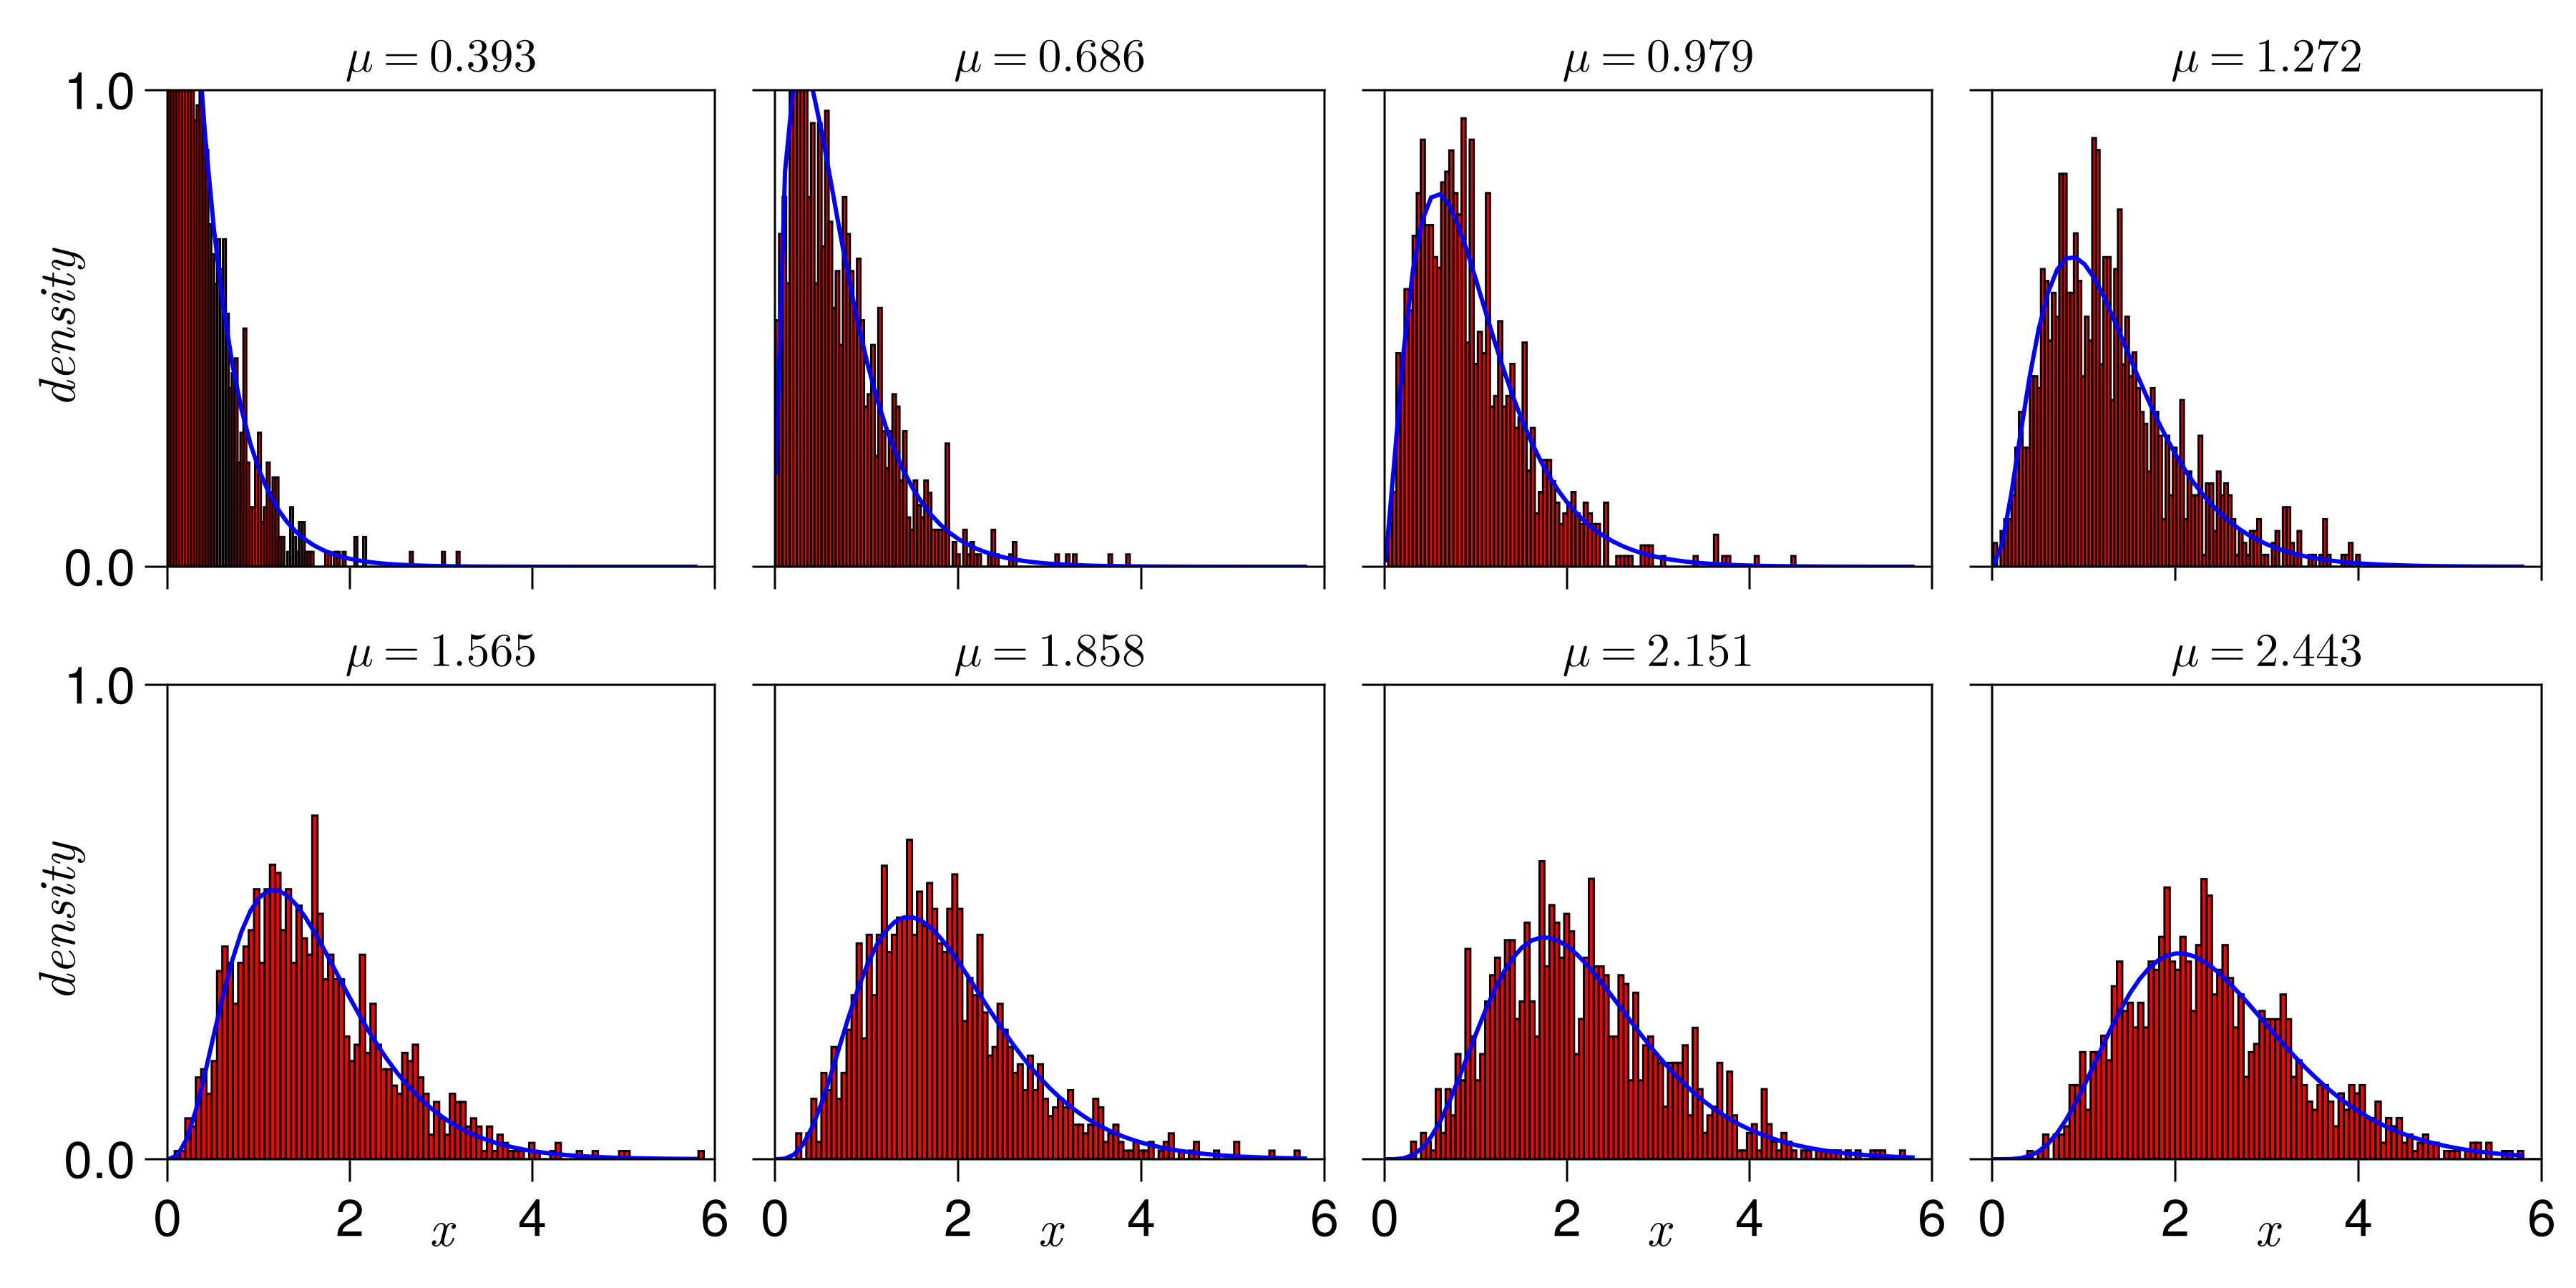
\includegraphics[keepaspectratio, width = \linewidth]{../figures/fig3.7.1.png}
                \label{fig3.7.1}
                \caption{}
        \end{subfigure}
        \newpage
        \begin{subfigure}[b]{0.95\textwidth}
                \centering 
                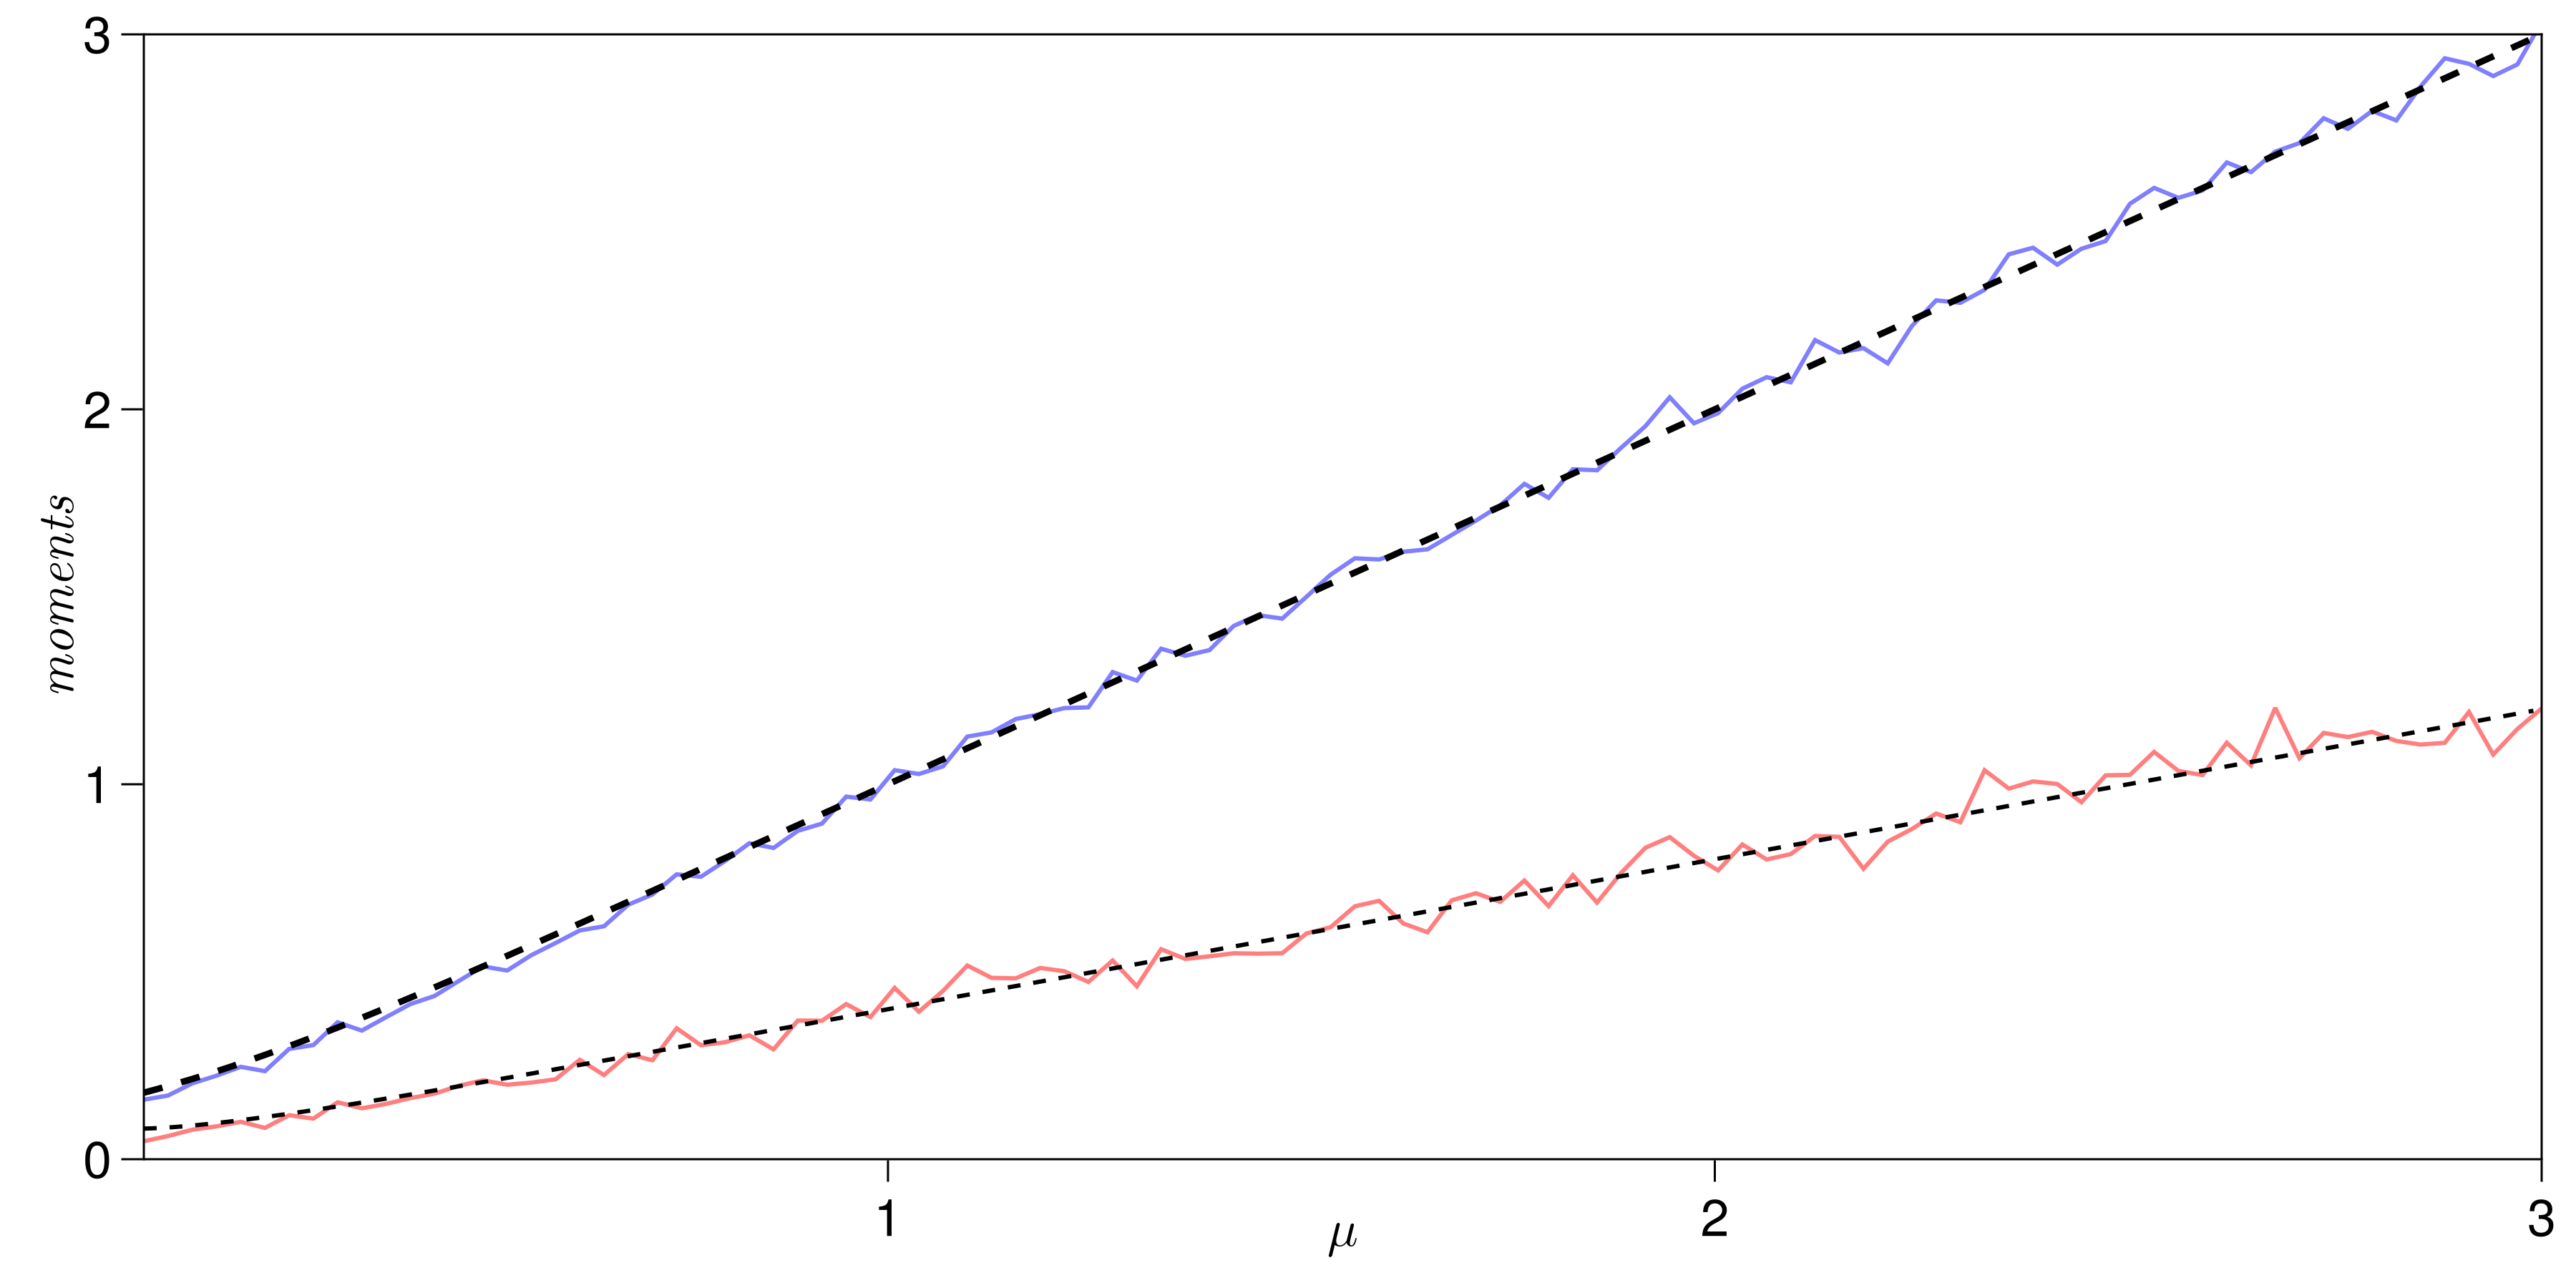
\includegraphics[keepaspectratio, width = \linewidth]{../figures/fig3.7.2.png}
                \label{fig3.7.2}
                \caption{}
        \end{subfigure}
         \caption{(a) Snapshots of the stationary Fokker-Plank distribution $p_{s}(x)$ (solid blue lines) for the transcritical normal form with multiplicative noise scaled by $\sigma = \sqrt{0.8}$ at different values of the parameter overlayed with histograms (red bars) associated to an ensemble simulation of $1000$ sample paths. (b) Comparison between the analytical parameter variation of the mean and variance of the stationary FPE (dashed black lines) with the sample estimates from the ensemble trajectories (ensemble average in blue while variance is in red).}
         \label{fig3.7}
\end{figure}
\end{example_continued}
\end{document}
